%%%%%%%%%%%%%%%%%%%%%%%%%%%%%%%%%%%%%%%%%
% Beamer Presentation
% LaTeX Template
% Version 1.0 (10/11/12)
%
% This template has been downloaded from:
% http://www.LaTeXTemplates.com
%
% License:
% CC BY-NC-SA 3.0 (http://creativecommons.org/licenses/by-nc-sa/3.0/)
%
%%%%%%%%%%%%%%%%%%%%%%%%%%%%%%%%%%%%%%%%%

%----------------------------------------------------------------------------------------
%	PACKAGES AND THEMES
%----------------------------------------------------------------------------------------

\documentclass{beamer}

\mode<presentation> {

% The Beamer class comes with a number of default slide themes
% which change the colors and layouts of slides. Below this is a list
% of all the themes, uncomment each in turn to see what they look like.

%\usetheme{default}
%\usetheme{AnnArbor}
%\usetheme{Antibes}
%\usetheme{Bergen}
%\usetheme{Berkeley}
%\usetheme{Berlin}
%\usetheme{Boadilla}
%\usetheme{CambridgeUS}
%\usetheme{Copenhagen}
%\usetheme{Darmstadt}
%\usetheme{Dresden}
%\usetheme{Frankfurt}
%\usetheme{Goettingen}
%\usetheme{Hannover}
%\usetheme{Ilmenau}
%\usetheme{JuanLesPins}
%\usetheme{Luebeck}
\usetheme{Madrid}
%\usetheme{Malmoe}
%\usetheme{Marburg}
%\usetheme{Montpellier}
%\usetheme{PaloAlto}
%\usetheme{Pittsburgh}
%\usetheme{Rochester}
%\usetheme{Singapore}
%\usetheme{Szeged}
%\usetheme{Warsaw}

% As well as themes, the Beamer class has a number of color themes
% for any slide theme. Uncomment each of these in turn to see how it
% changes the colors of your current slide theme.

%\usecolortheme{albatross}
%\usecolortheme{beaver}
%\usecolortheme{beetle}
%\usecolortheme{crane}
%\usecolortheme{dolphin}
%\usecolortheme{dove}
%\usecolortheme{fly}
%\usecolortheme{lily}
%\usecolortheme{orchid}
%\usecolortheme{rose}
%\usecolortheme{seagull}
%\usecolortheme{seahorse}
%\usecolortheme{whale}
%\usecolortheme{wolverine}

%\setbeamertemplate{footline} % To remove the footer line in all slides uncomment this line
%\setbeamertemplate{footline}[page number] % To replace the footer line in all slides with a simple slide count uncomment this line

%\setbeamertemplate{navigation symbols}{} % To remove the navigation symbols from the bottom of all slides uncomment this line
}

\usepackage{graphicx} % Allows including images
\usepackage{booktabs} % Allows the use of \toprule, \midrule and \bottomrule in tables

%----------------------------------------------------------------------------------------
%	TITLE PAGE
%----------------------------------------------------------------------------------------

\title[]{Wave Generation and Propagation in an Underwater Energy Release} % The short title appears at the bottom of every slide, the full title is only on the title page

\author{Rahul Joshi} % Your name
 
\institute[IIT, Bombay] % Your institution as it will appear on the bottom of every slide, may be shorthand to save space
{
Under the Guidance of \\ Prof. Shivasubramanian Gopalakrishnan \\\vspace{0.2cm}Department of Mechanical Engineering \\ Indian Institute of Technology, Bombay% Your institution for the title page
\medskip
}

\date{\today} % Date, can be changed to a custom date

\titlegraphic{
\includegraphics[width=2cm]{iitb.jpg}}

\begin{document}

\begin{frame}
\titlepage % Print the title page as the first slide
\end{frame}

\begin{frame}
\frametitle{Overview} % Table of contents slide, comment this block out to remove it
\tableofcontents % Throughout your presentation, if you choose to use \section{} and \subsection{} commands, these will automatically be printed on this slide as an overview of your presentation
\end{frame}

%----------------------------------------------------------------------------------------
%	PRESENTATION SLIDES
%----------------------------------------------------------------------------------------
\section{Introduction to Underwater Energy Release}

\begin{frame}
\frametitle{Introduction to Underwater Energy Release}
\begin{itemize}
  \item Underwater Energy Release is an phenomena which occurs due to detonation under water surface 
  \item The energy release is classified into two type, depending on \textbf{$\frac{d}{W^\frac{1}{3}}$ }: \\
  $\rightarrow$ Amount of TNT or explosive 'W' (lbs) \\
  $\rightarrow$ Depth 'd' (ft) at which the energy release has taken place
  \item Deep water energy release : $\frac{d}{W^\frac{1}{3}} > 16$  
  \item Shallow water energy release : $\frac{d}{W^\frac{1}{3}} < 3$ 
  \item Now depending on the depth at which the energy release takes place the nature of the water waves varies
\end{itemize}

\end{frame}

%-----------------INITIAL CONDITIONS-------------------------------

%\section{Initial conditions}
\begin{frame}
\frametitle{Initial Condition}
\begin{figure}[h]  
\begin{center}  
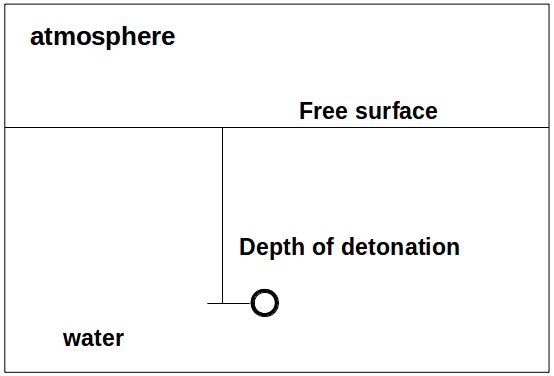
\includegraphics[scale=0.4]{1.png}
\caption{\tiny{Schematic representation of initial condition of underwater energy release}}
\end{center}  
\end{figure}
\end{frame}

%----------------SHOCK WAVE GENERATION--------------------------------

%\section{Shock Wave generation}
\begin{frame}
\frametitle{Shock Wave generation}
\begin{figure}[h]  
\begin{center}  
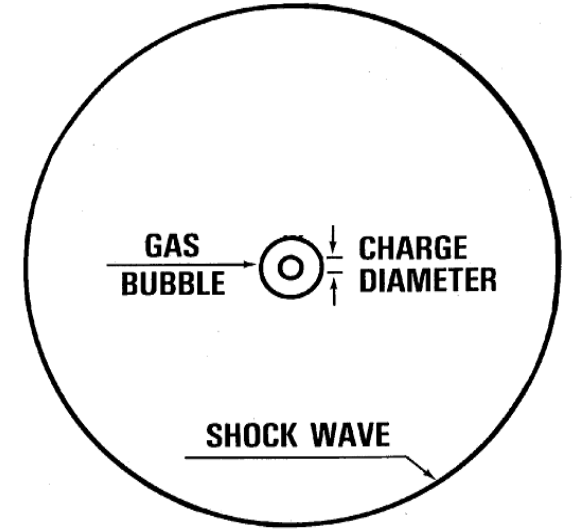
\includegraphics[scale=0.15]{2.png}
\caption{\tiny{Shock wave and center gas bubble after detonation}}
\end{center}  
\end{figure}
\begin{itemize}
  \item \small In majority of underwater energy release the shock wave is the main cause of damage 
  \item \small Initial shock wave is propagated in milliseconds and the corresponding bubble contraction and expansion is occurs in seconds 
  \item \small Due to the reflection of the shock waves from the free surface, a change in the pressure field is also observed.
\end{itemize}
\end{frame}

%------------------CAVITATION------------------------------

\begin{frame}
\frametitle{Cavitation}
\begin{figure}[h]  
\begin{center}  
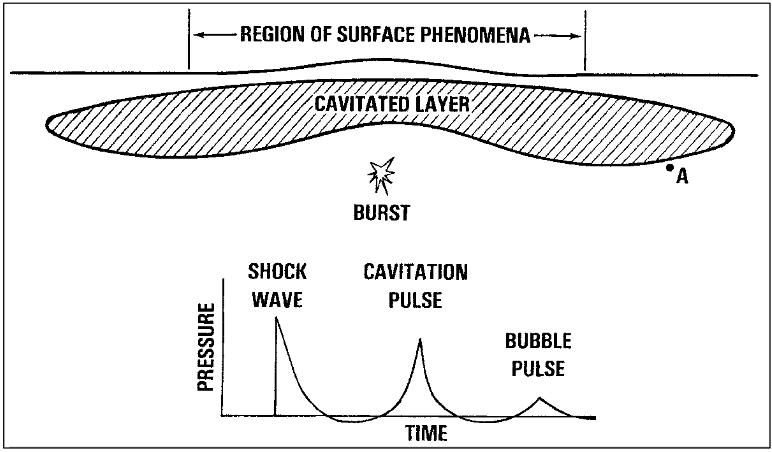
\includegraphics[scale=0.20]{3.png}
\caption{\tiny{Cavitation after energy release}}
\end{center}  
\end{figure}

\begin{itemize}
  \item As the shock wave is generated it travels to surface and reflects back as a tensile wave
  \item Since water cannot sustain this large amount of tensile force it leads to cavitation
  \item Due to the effects of gravity and atmospheric pressure this region of cavitation and bubble from the bottom surface collide and give rise to a \textbf{Water Hammer Effect}
\end{itemize}
\end{frame}


%--------------------GAS BUBBLE DYNAMICS ----------------------------
\section{Gas Bubble Dynamics}
\begin{frame}
\frametitle{Gas Bubble Dynamics}
\begin{figure}[h]  
\begin{center}  
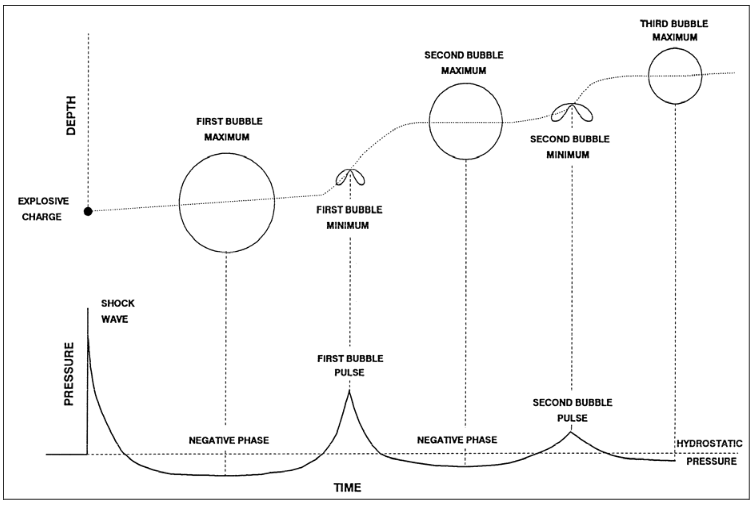
\includegraphics[scale=0.350]{4.png}
\caption{\tiny{Different phases of Explosion bubble with pressure-time graph}}
\end{center}  
\end{figure}
\end{frame}

%----------------------GOVERNING EQUATIONS-------------------------------------

\section{Governing Equations}
\begin{frame}
\frametitle{Governing Equations}
\begin{itemize}
  \item Pressure on bubble surface $\rightarrow$ \boxed {$$P_{R} = 7.8\frac{W}{V}^{\gamma}+\sigma$$}\\
  \item Initial radius of the bubble $\rightarrow$ \boxed {$$R_{m} = 3.38( \frac{W}{H+10})^{\frac{1}{3}} $$} \\
  \item We neglect viscosity and surface tension effects
  \item 

\end{itemize}

\end{frame}

%------------------------------------------------

\begin{frame} % Need to use the fragile option when verbatim is used in the slide
\frametitle{Governing Equations}

\end{frame}

%--------------------VoF METHOD----------------------------

\section{Volume of Fluid (VoF)}
\begin{frame}
\frametitle{Volume of Fluid}
\begin{itemize}
  \item Volume of Fluid (VoF), is one of the numerical technique for tracking and locating free surfaces or a two fluid interface
  \item Type of advection scheme which is used to track the motion and shape of the interface
  \begin{figure}[h]  
  \begin{center}  
  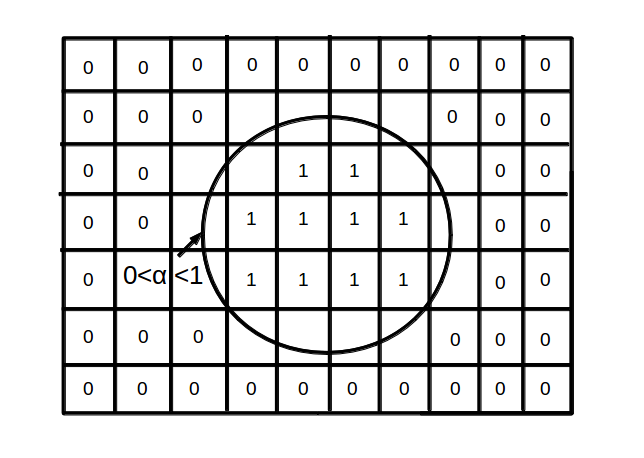
\includegraphics[scale=0.25]{5.png}
  \caption{\tiny{Volume fraction $\alpha$ for a Fluid-gas interface}}
  \end{center}  
  \end{figure}
  \item $\alpha = \frac{V_{k}}{V_{T}}$
\end{itemize}

\end{frame}

%------------------------------------------------

\begin{frame}
\frametitle{Volume of Fluid- Interface reconstruction}
\begin{figure}[h]  
\begin{center}  
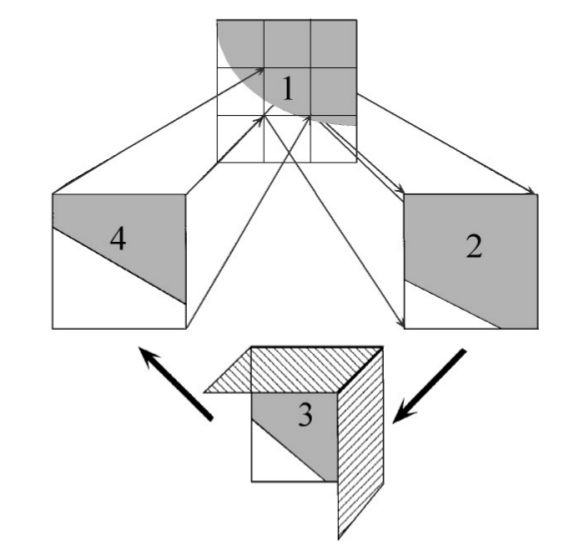
\includegraphics[scale=0.28]{6.png}
\caption{\tiny VoF interface reconstruction }
\end{center}  
\end{figure}

\end{frame}

%--------------------OPENFOAM----------------------------
\section{OpenFOAM}
\begin{frame}
\frametitle{OpenFOAM}
\begin{figure}[h]  
\begin{center}  
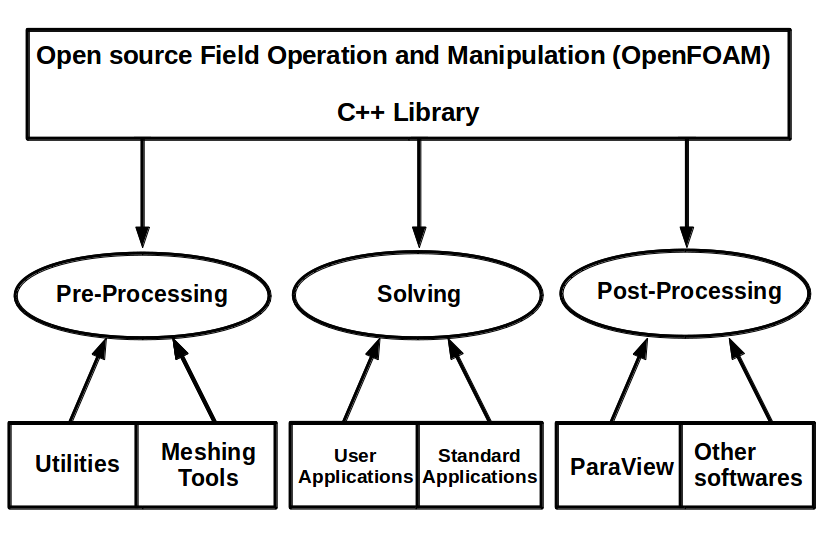
\includegraphics[scale=0.25]{7.png}
\caption{\tiny Overview of OpenFOAM }
\end{center}  
\end{figure}

\end{frame}

%------------------------------------------------

\begin{frame}
\frametitle{OpenFOAM- File structure}
\begin{figure}[h]  
\begin{center}  
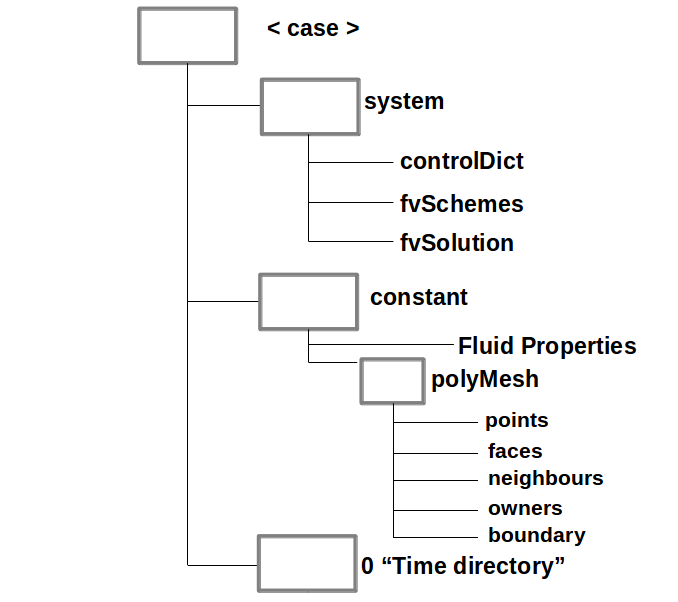
\includegraphics[scale=0.3]{8.png}
\caption{\tiny File structure of OpenFOAM }
\end{center}  
\end{figure}

\end{frame}

%----------------------------CONCLUSION------------------------------------------------------------
\section{Conclusion}
\begin{frame}
\frametitle{Conclusion}
\begin{itemize}
  \item Physics behind underwater energy release is both fascinating and challenging
  \item From literature it was found that there is scope for implementation of non-conservative form of the equations
  \item Quantify the resulting errors for energy release in free/ compact surfaces as well as in deep and shallow water depths
\end{itemize}
\end{frame}

%-------------------------FUTURE WORK -----------------------------------------------------------------

\section{Future Work Proposed}
\begin{frame}
\frametitle{Future Work}
\begin{itemize}
  \item Using OpenFOAM solve the test case given below and validate the results with the paper published by S.T.Miller et.al   
  \begin{figure}[h]  
  \begin{center}  
  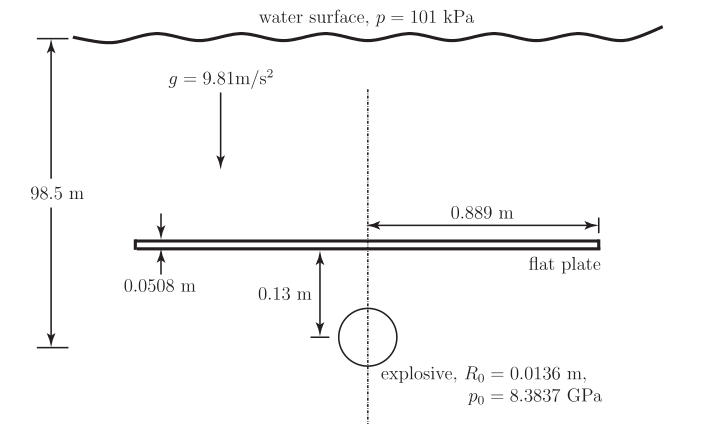
\includegraphics[scale=0.35]{9.png}
  \caption{\tiny Test case for validation,S.T. Miller et.al }
  \end{center}  
\end{figure}
  
\end{itemize}
\end{frame}

%-------------------REFRENCES-----------------------------------------------------------------------
\section{Refrences}
\begin{frame}
\frametitle{Refrences}
\end{frame}

%---------------------------END OF PPT-----------------------------------------------------------------

\end{document} 
